	\pagestyle{fancy}
	\setcounter{page}{1} 
	\fancyhead[LO,RE]{B-\thepage}
	\fancyhead[RO,LE]{Anhang B: Zeichnungen der Bauteile}
	\addcontentsline{toc}{subparagraph}{Anhang B: Zeichnungen der Bauteile}
	\section*{Anhang B: Zeichnungen der Bauteile}
	
	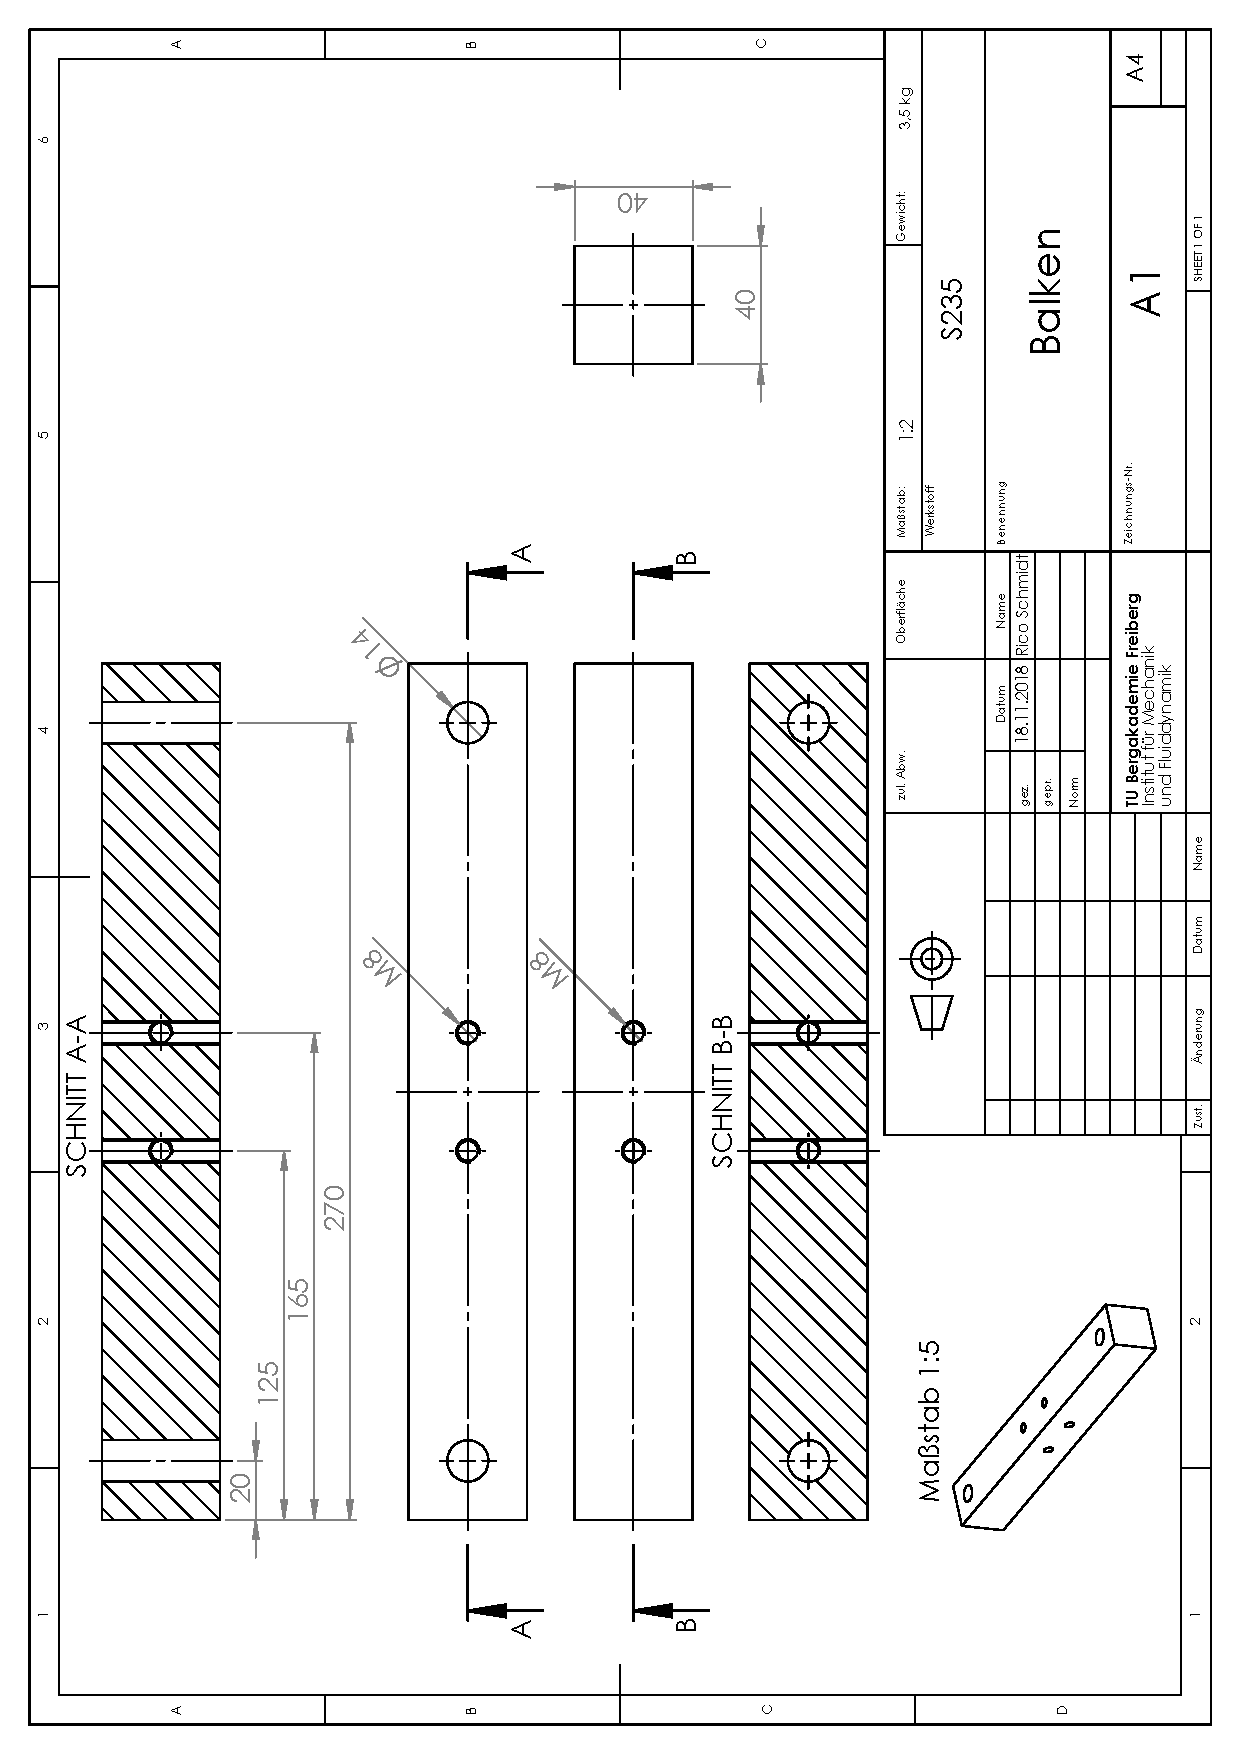
\includegraphics[angle=-90,width=1.0\textwidth]{Anhang/PDFs/Balken}
	
	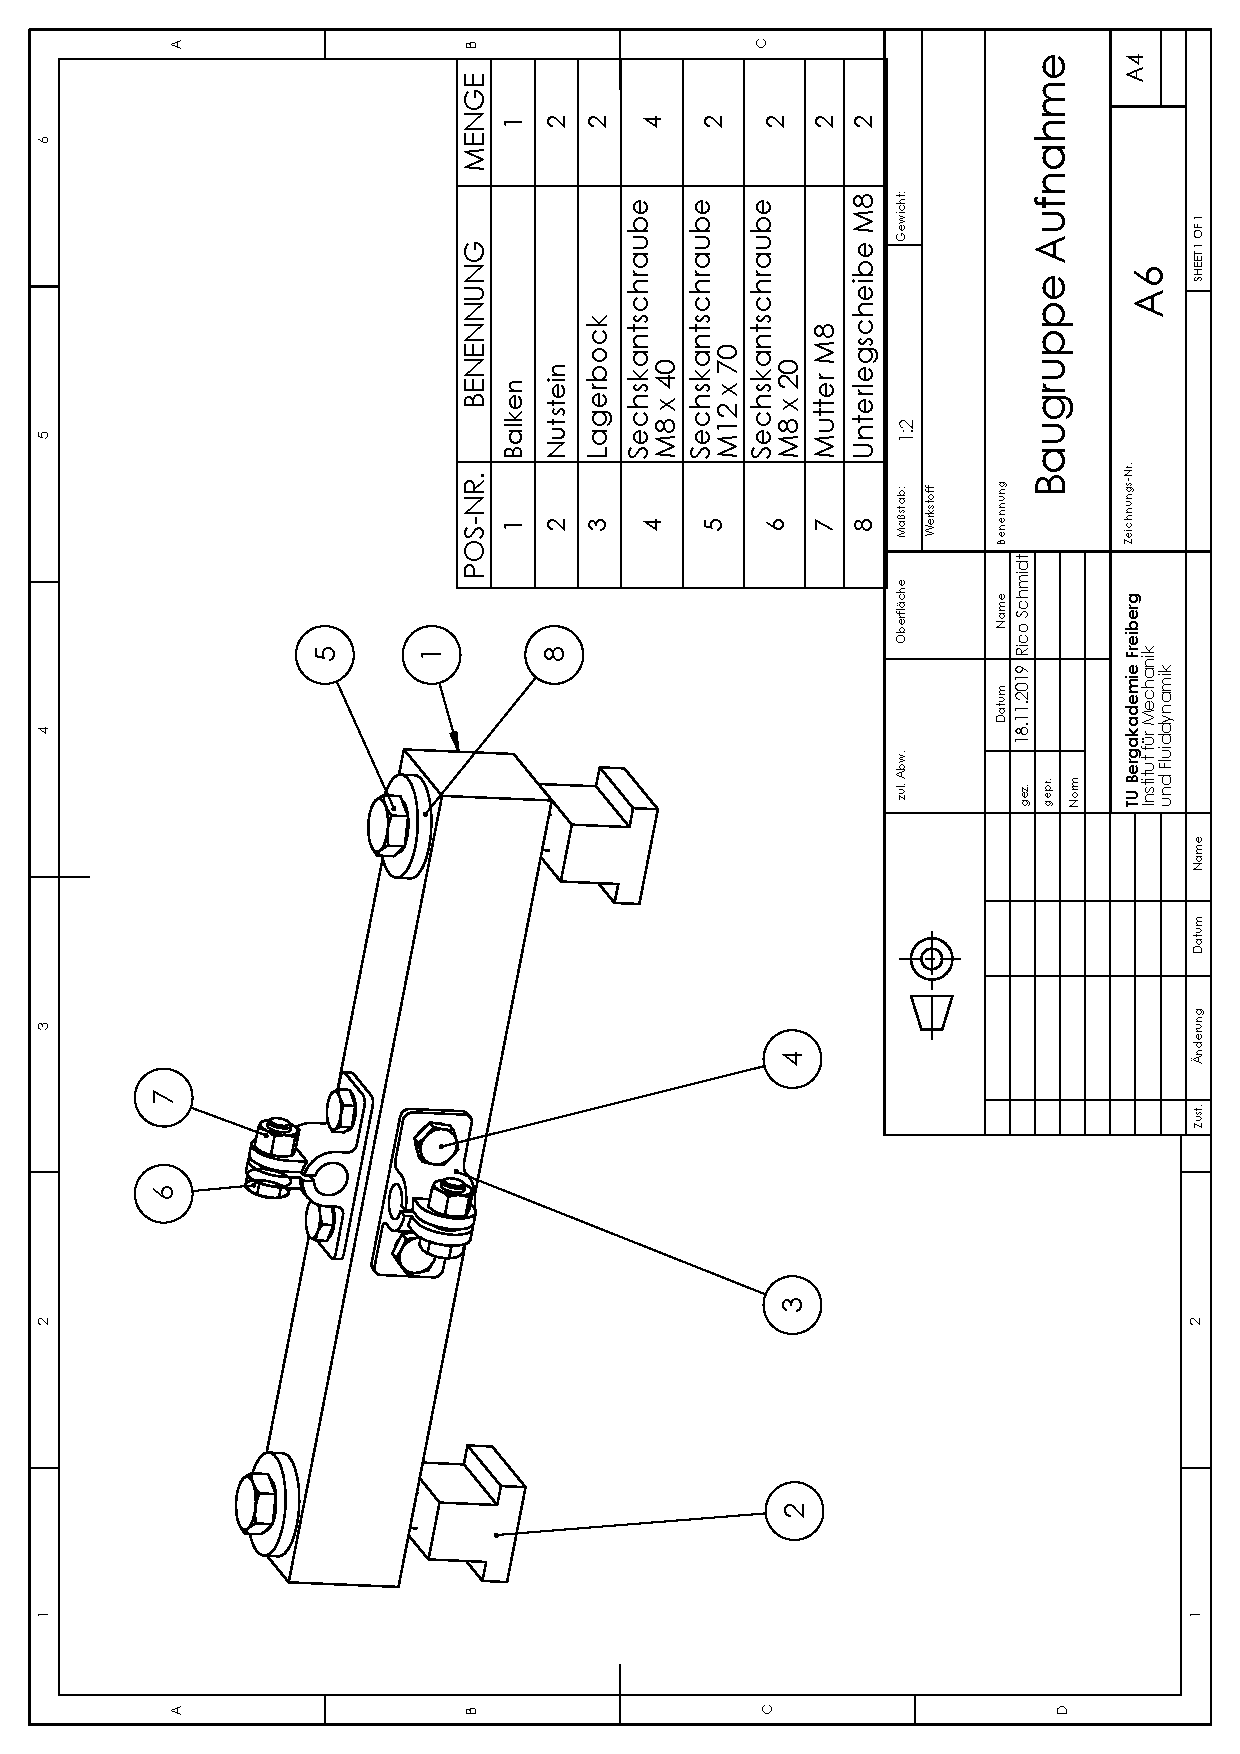
\includegraphics[angle=-90,width=1.0\textwidth]{Anhang/PDFs/Baugruppe_Aufnahme}
	
	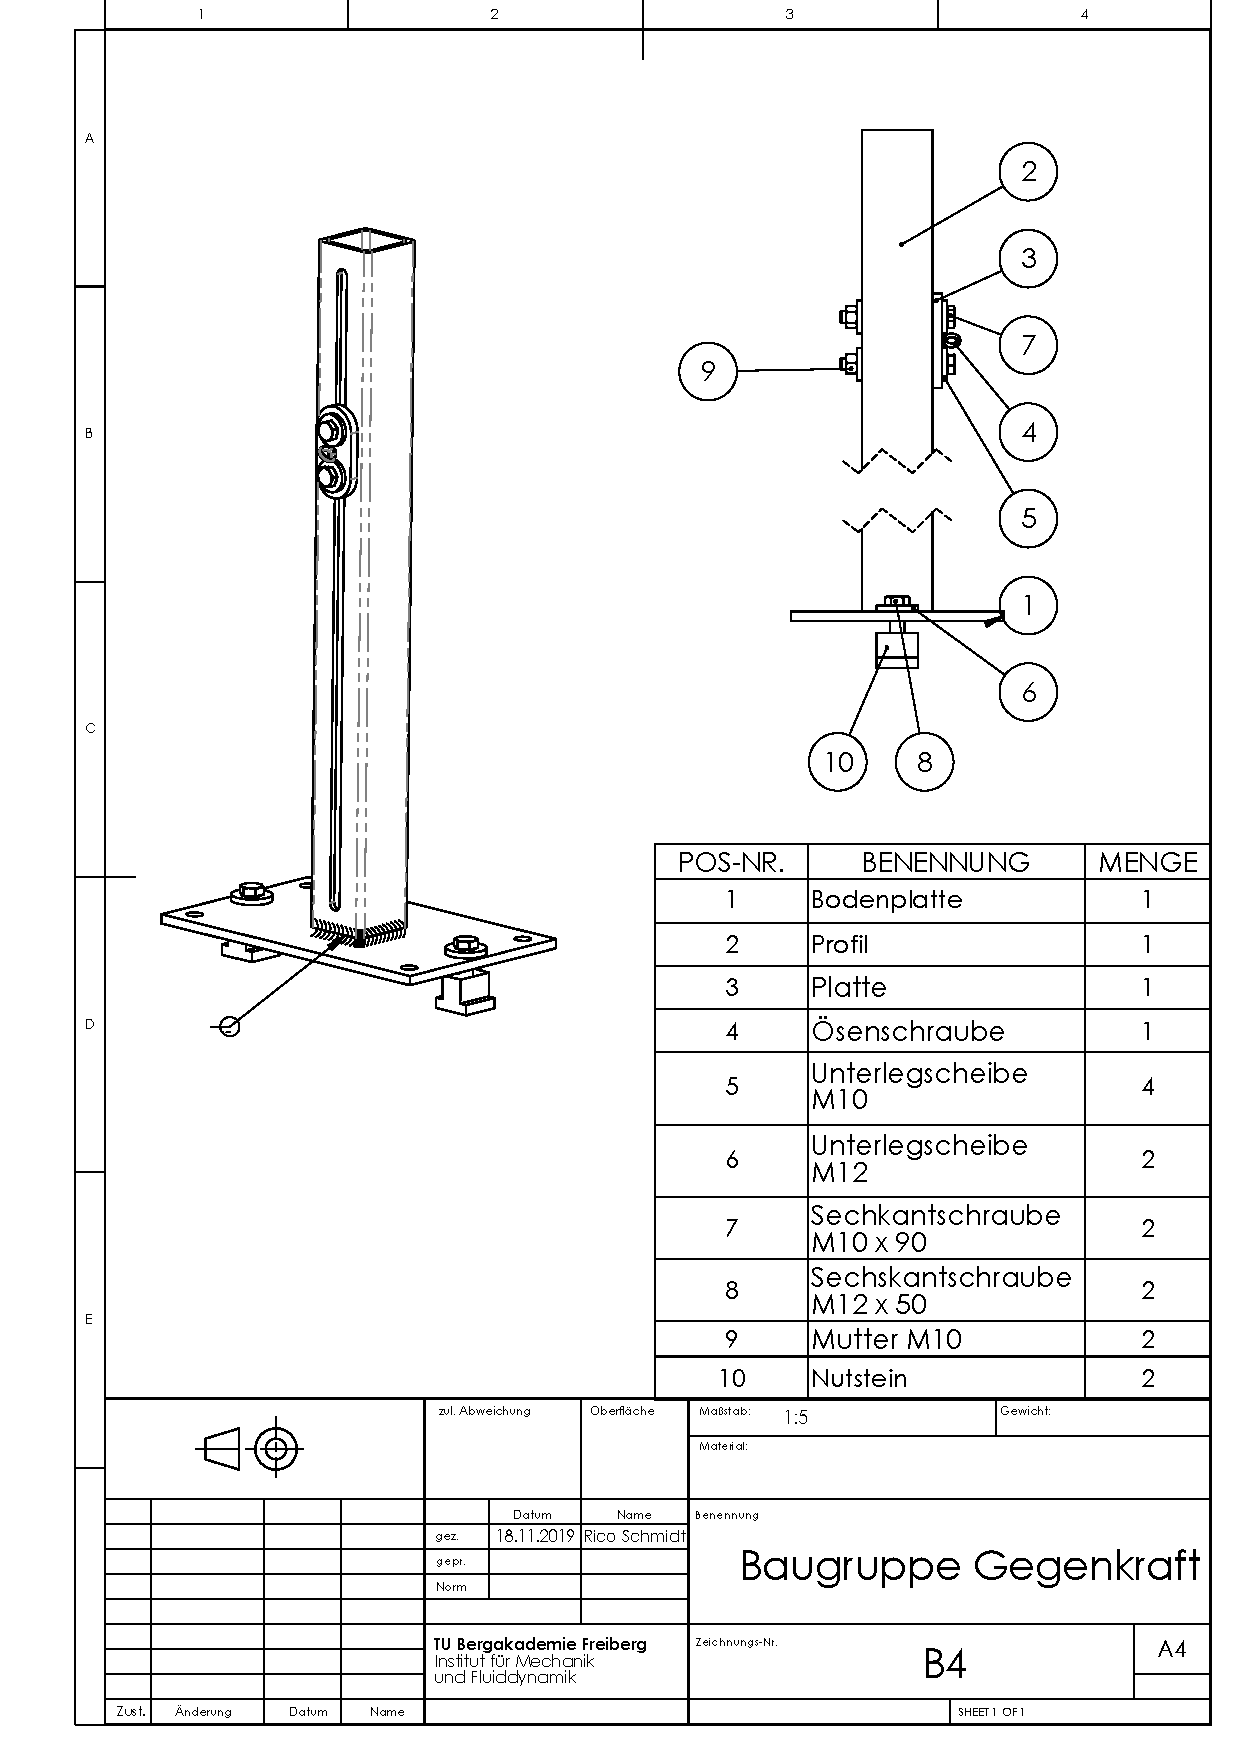
\includegraphics[angle=-90,width=1.0\textwidth]{Anhang/PDFs/Baugruppe_Gegenkraft}
	
	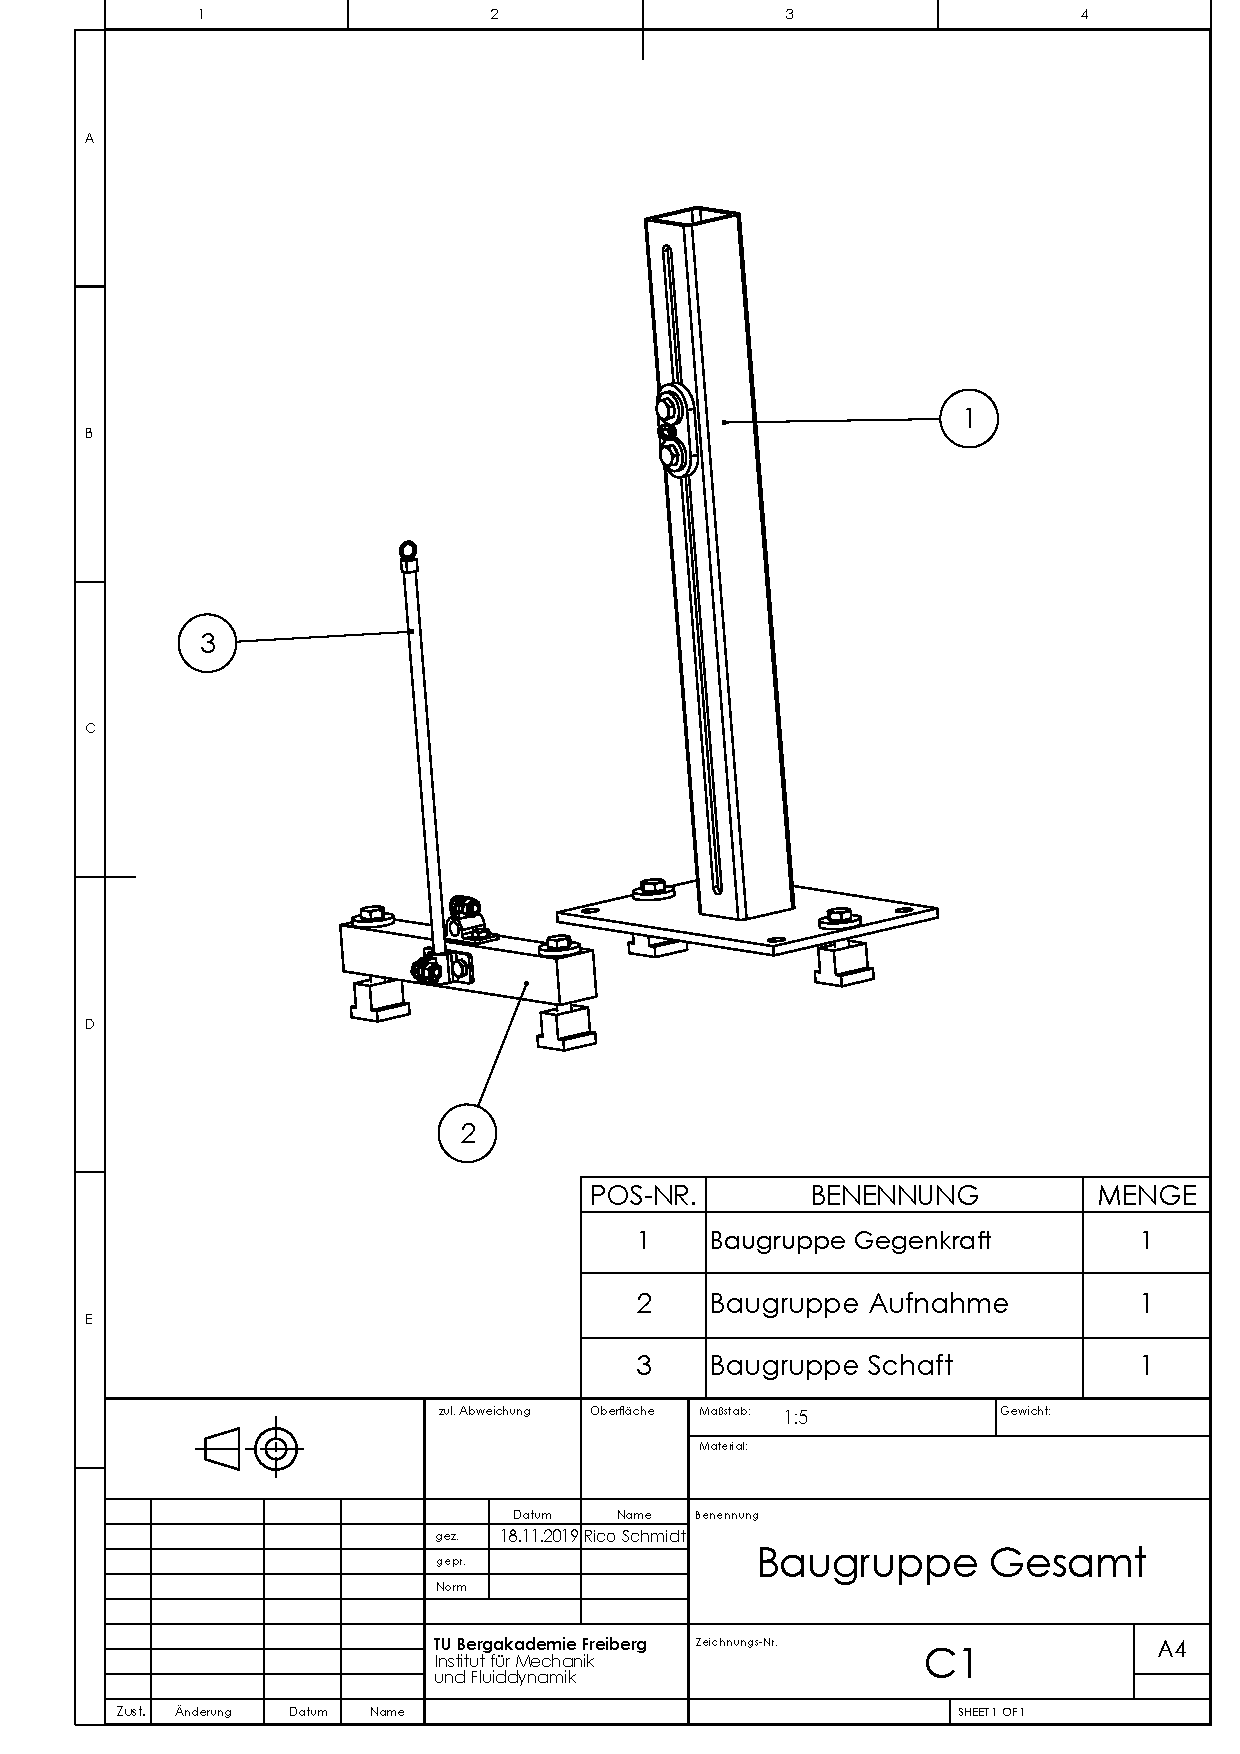
\includegraphics[angle=-90,width=1.0\textwidth]{Anhang/PDFs/Baugruppe_Gesamt}
	
	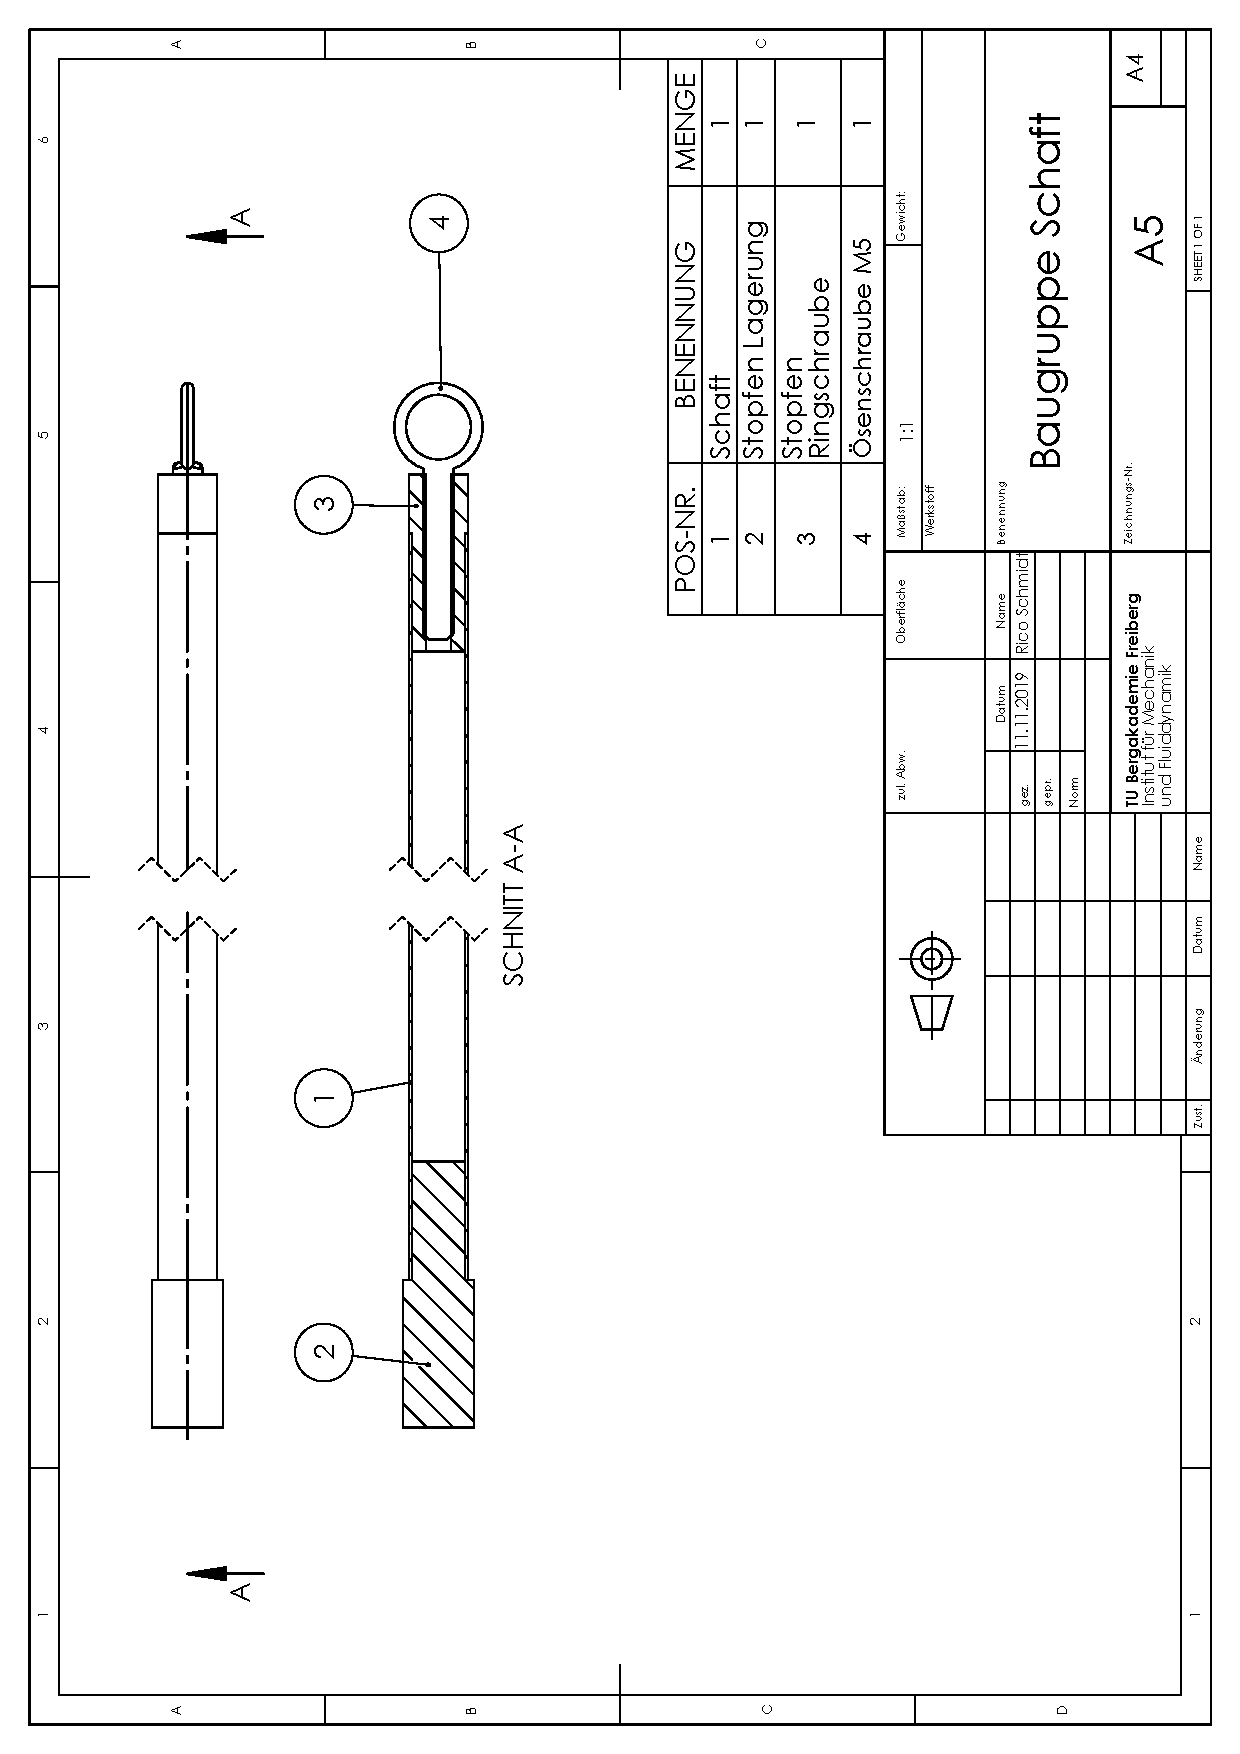
\includegraphics[angle=-90,width=1.0\textwidth]{Anhang/PDFs/Baugruppe_Schaft}
	
	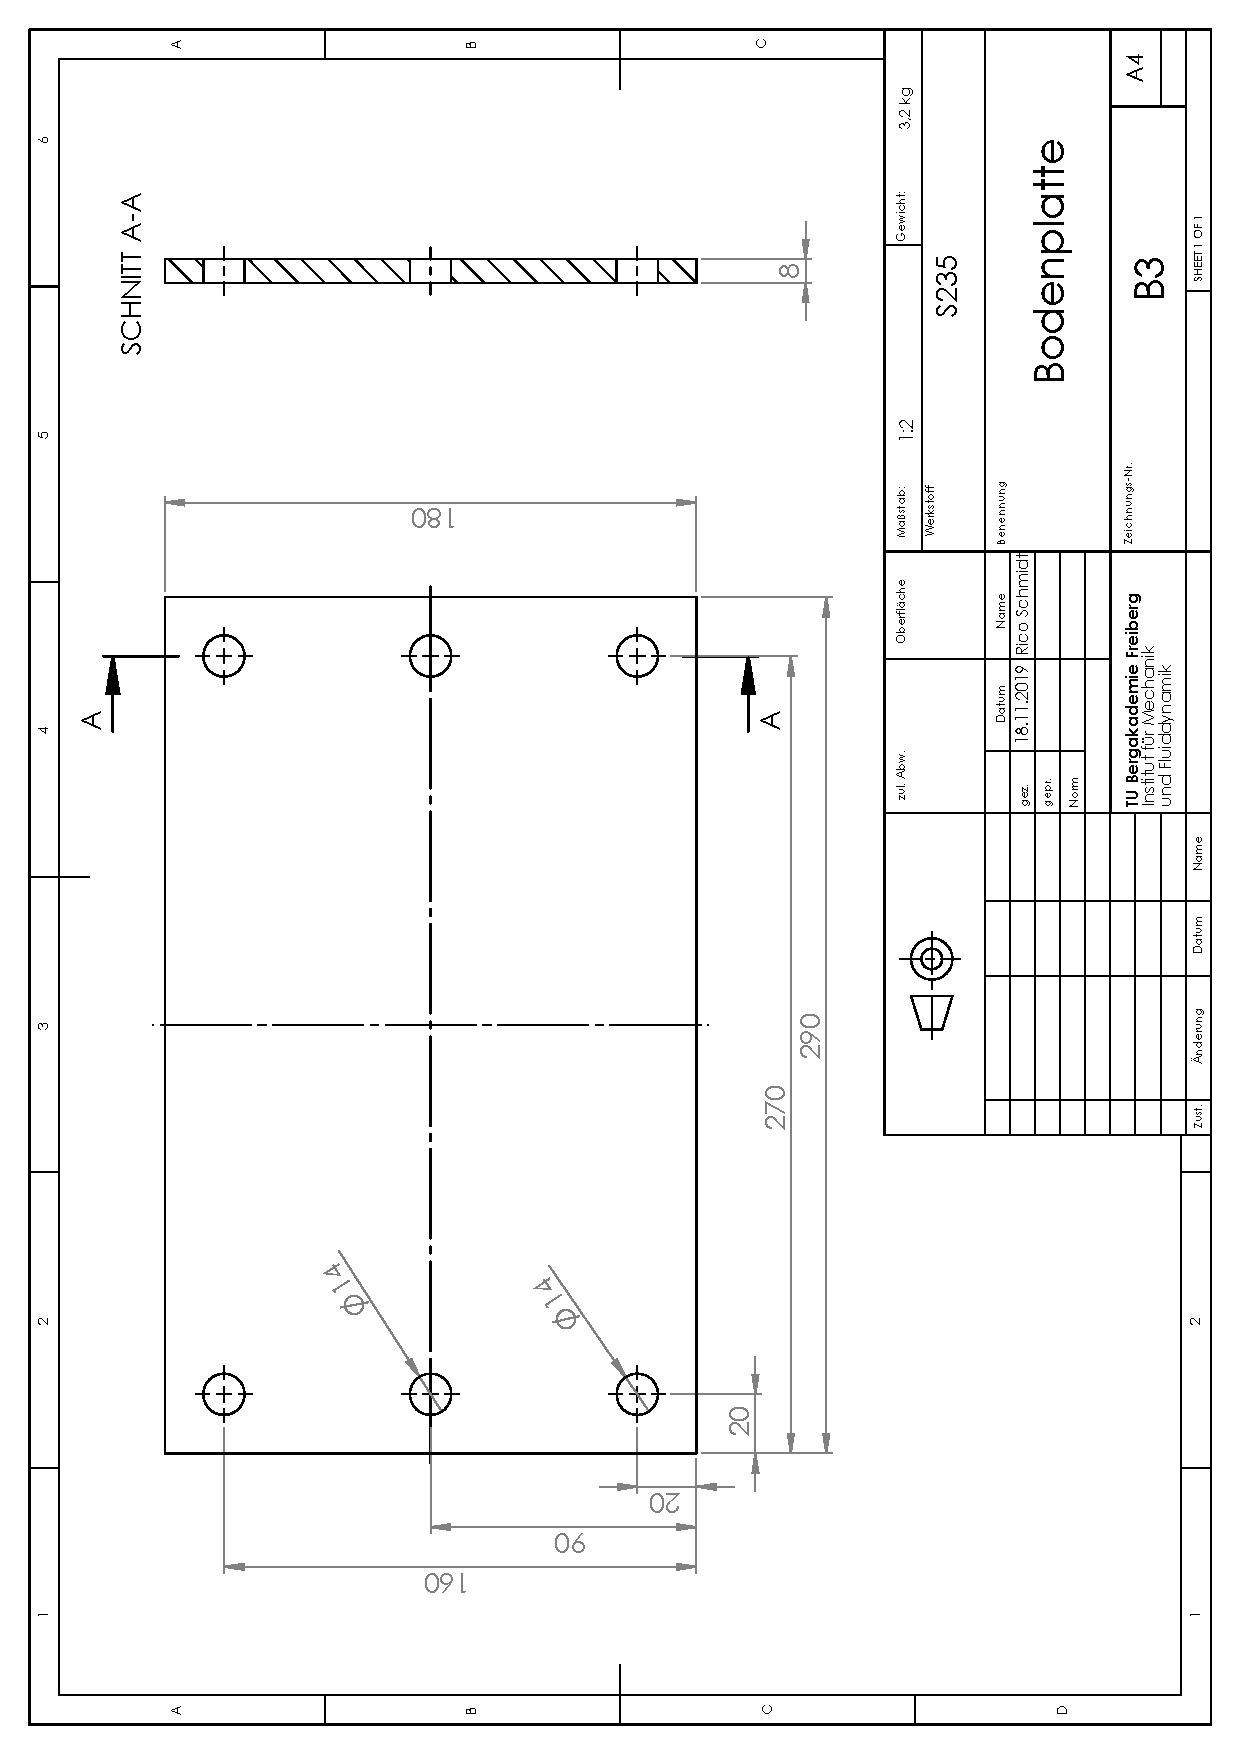
\includegraphics[angle=-90,width=1.0\textwidth]{Anhang/PDFs/Bodenplatte}
	
	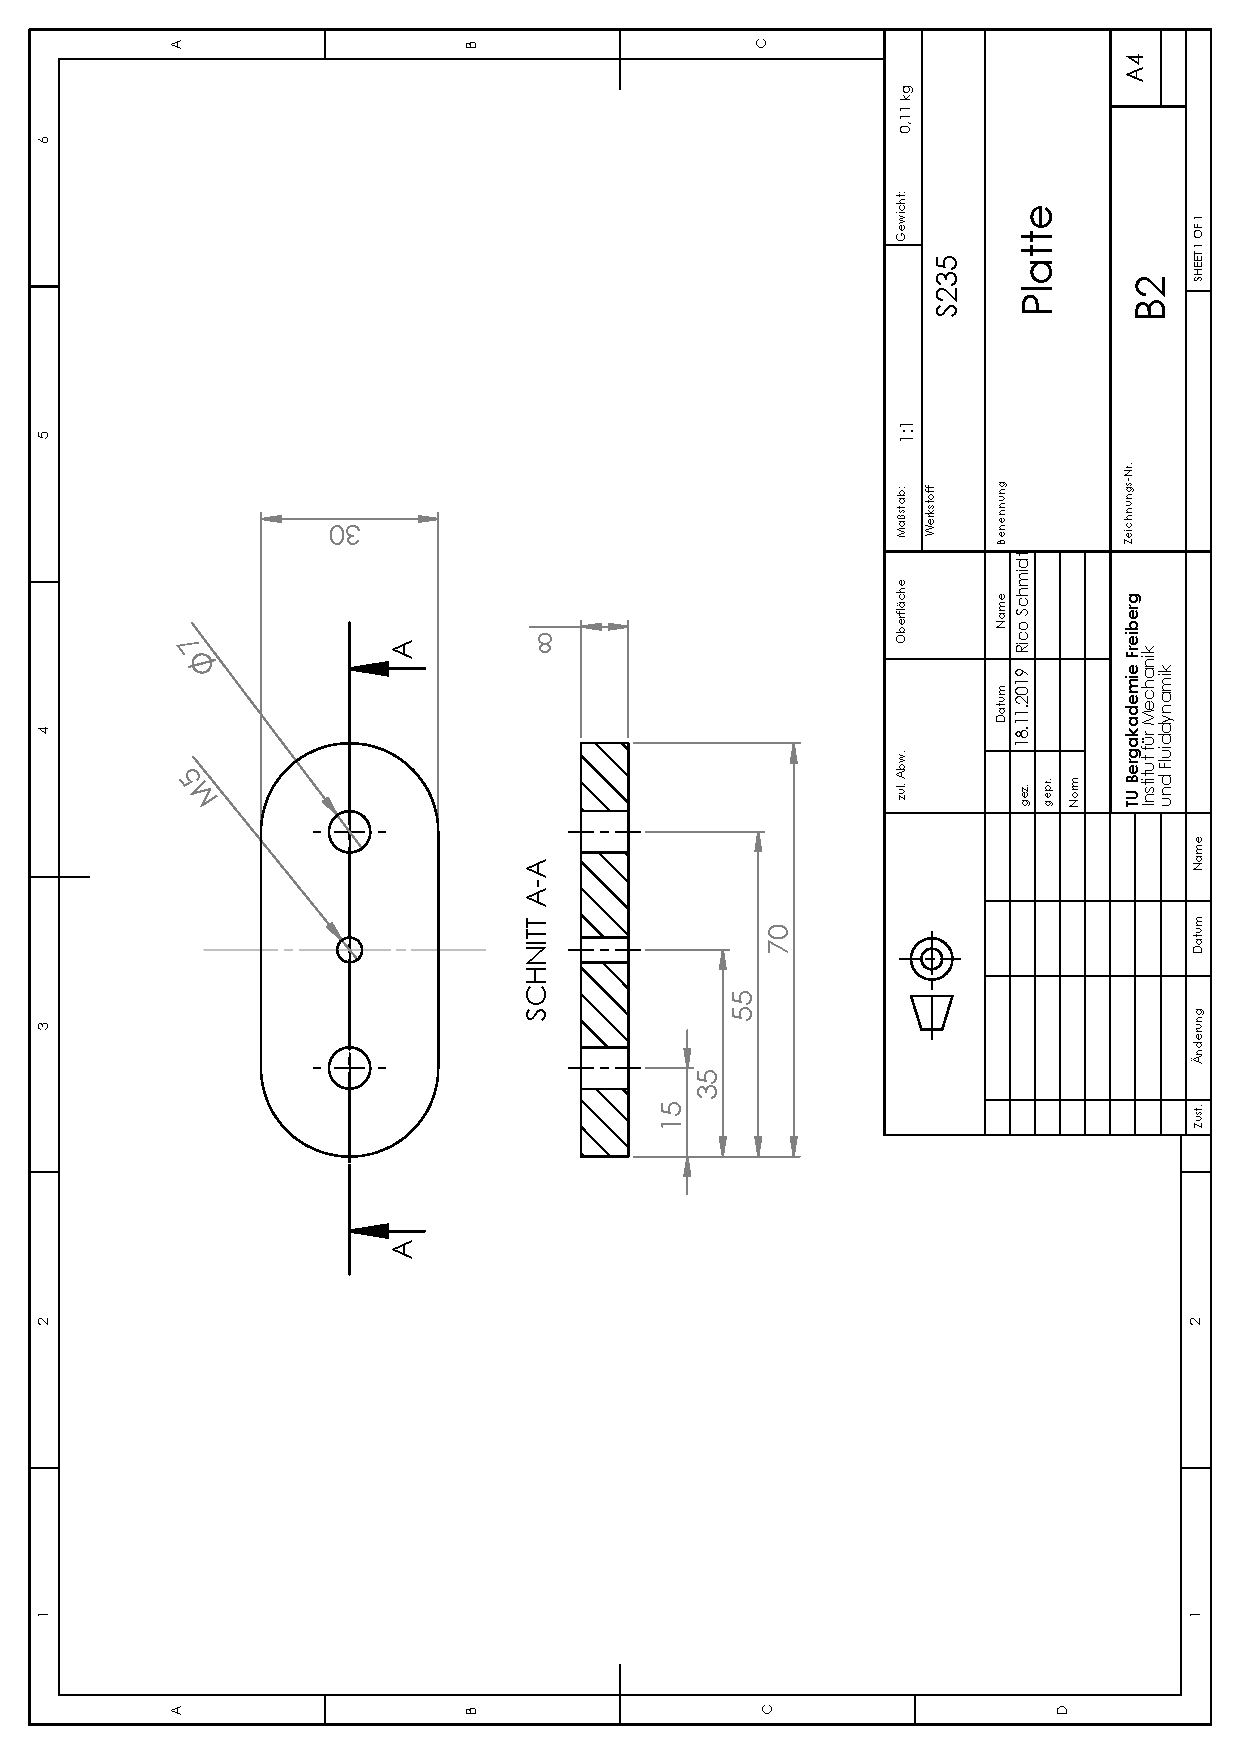
\includegraphics[angle=-90,width=1.0\textwidth]{Anhang/PDFs/Platte_Schlitte}
	
	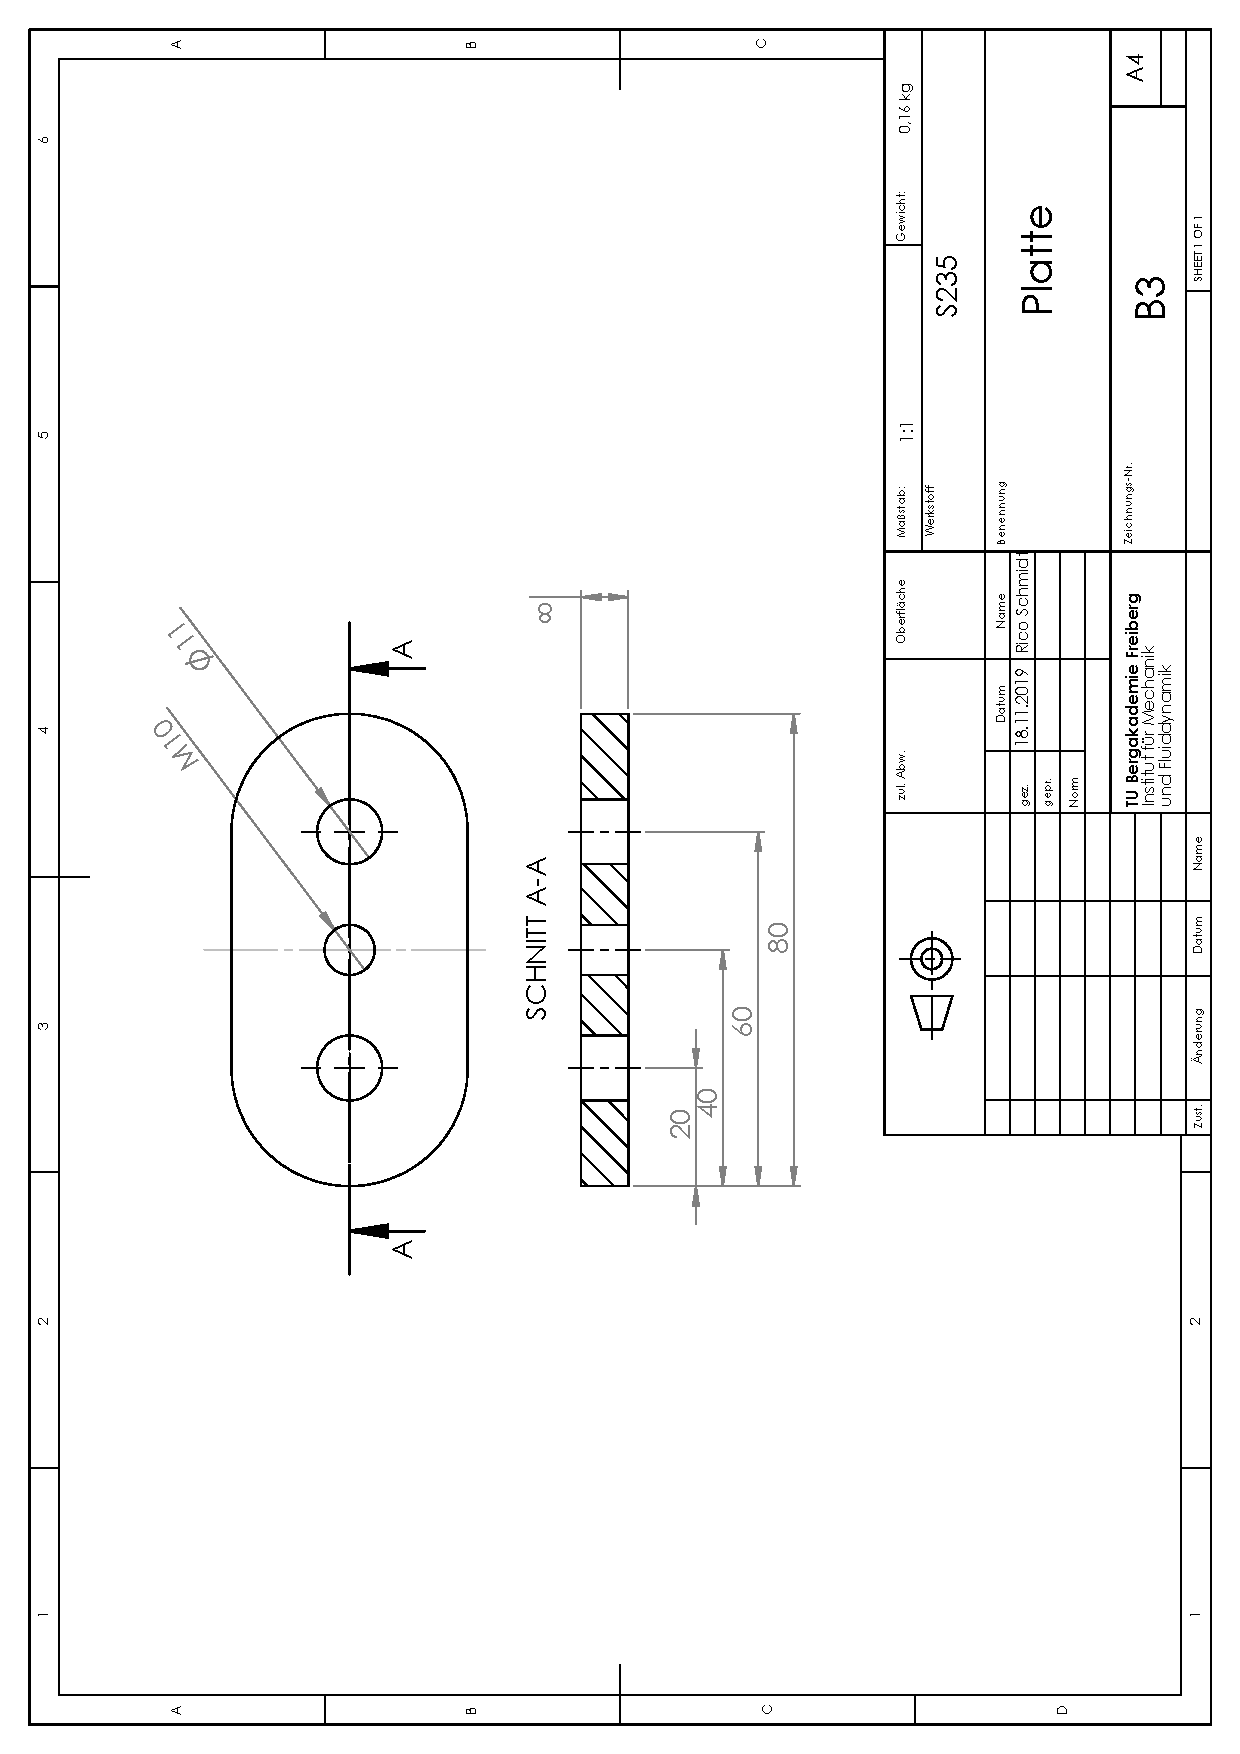
\includegraphics[angle=-90,width=1.0\textwidth]{Anhang/PDFs/Platte_Schlitten}
	
	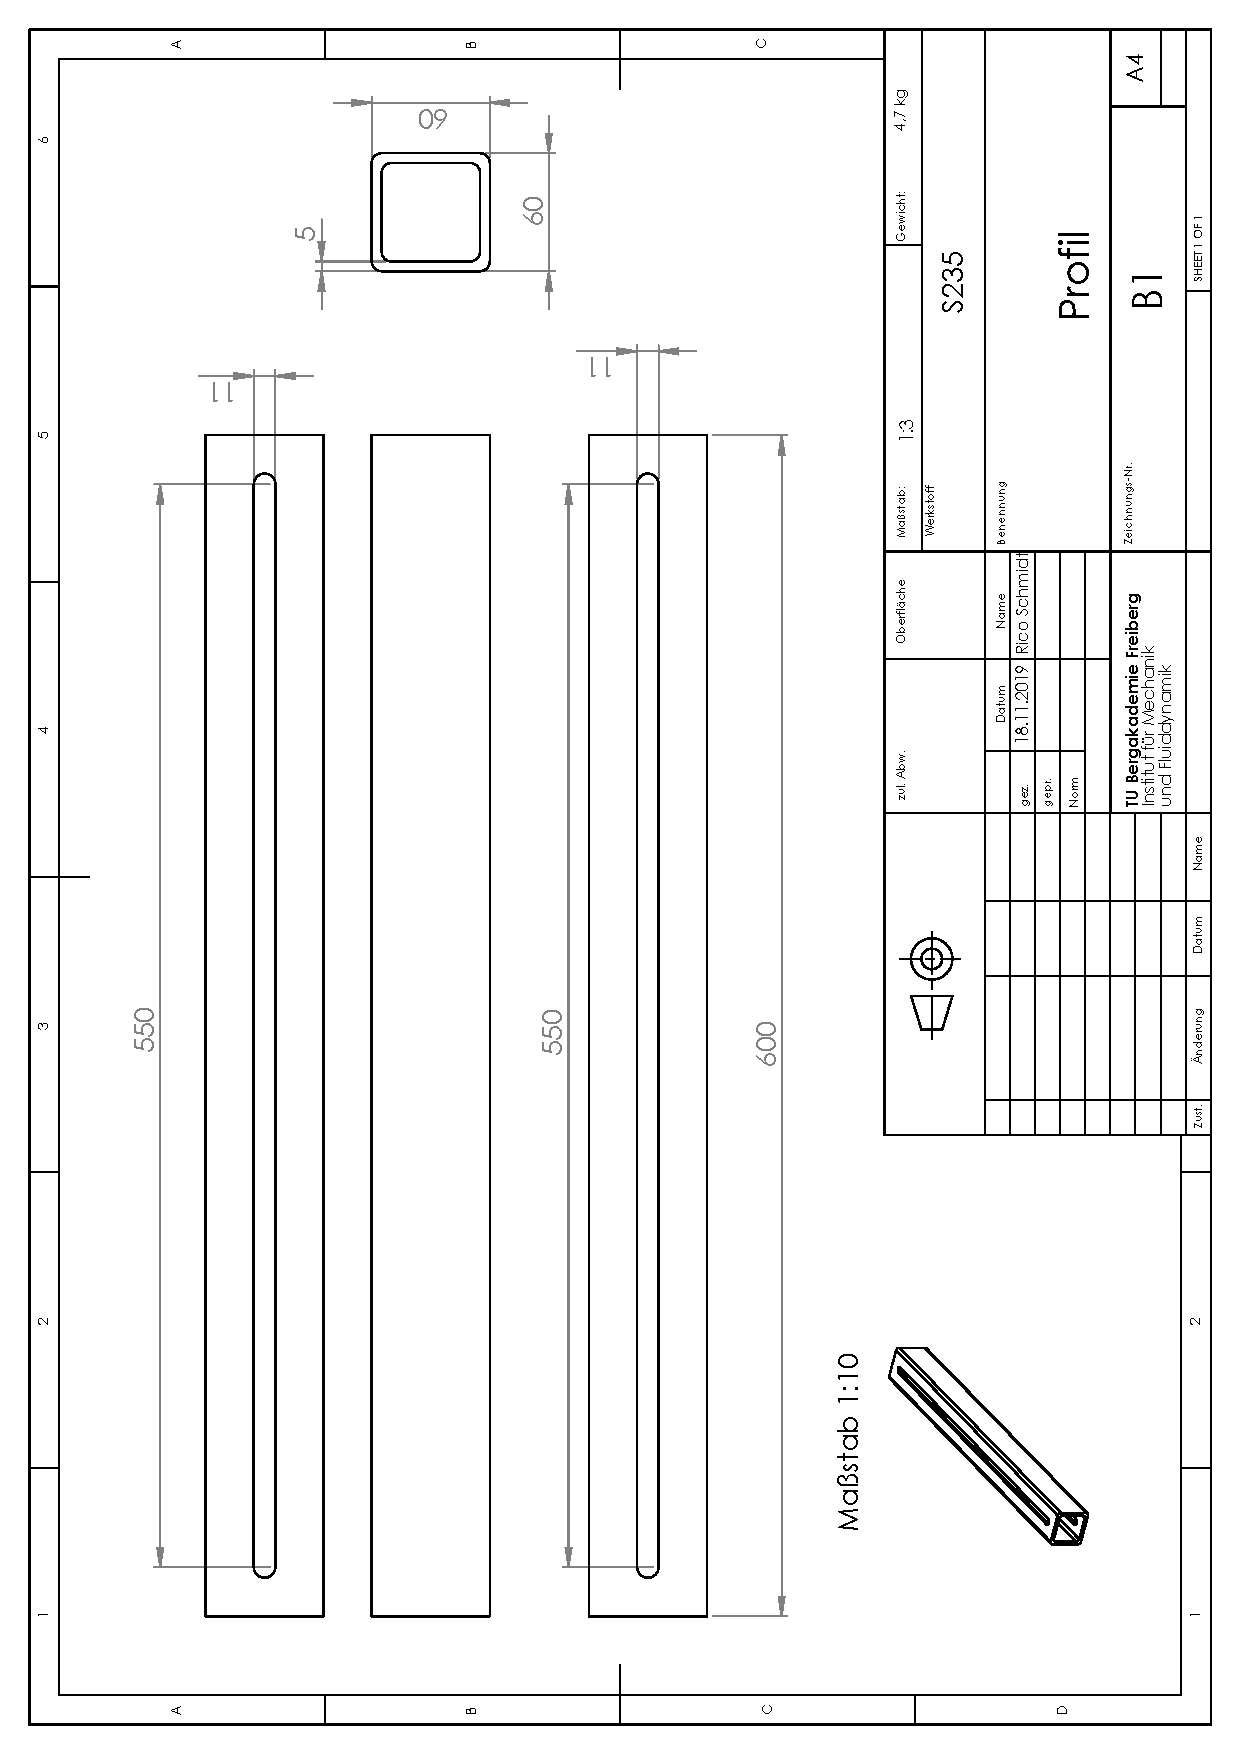
\includegraphics[angle=-90,width=1.0\textwidth]{Anhang/PDFs/Profil}
	
	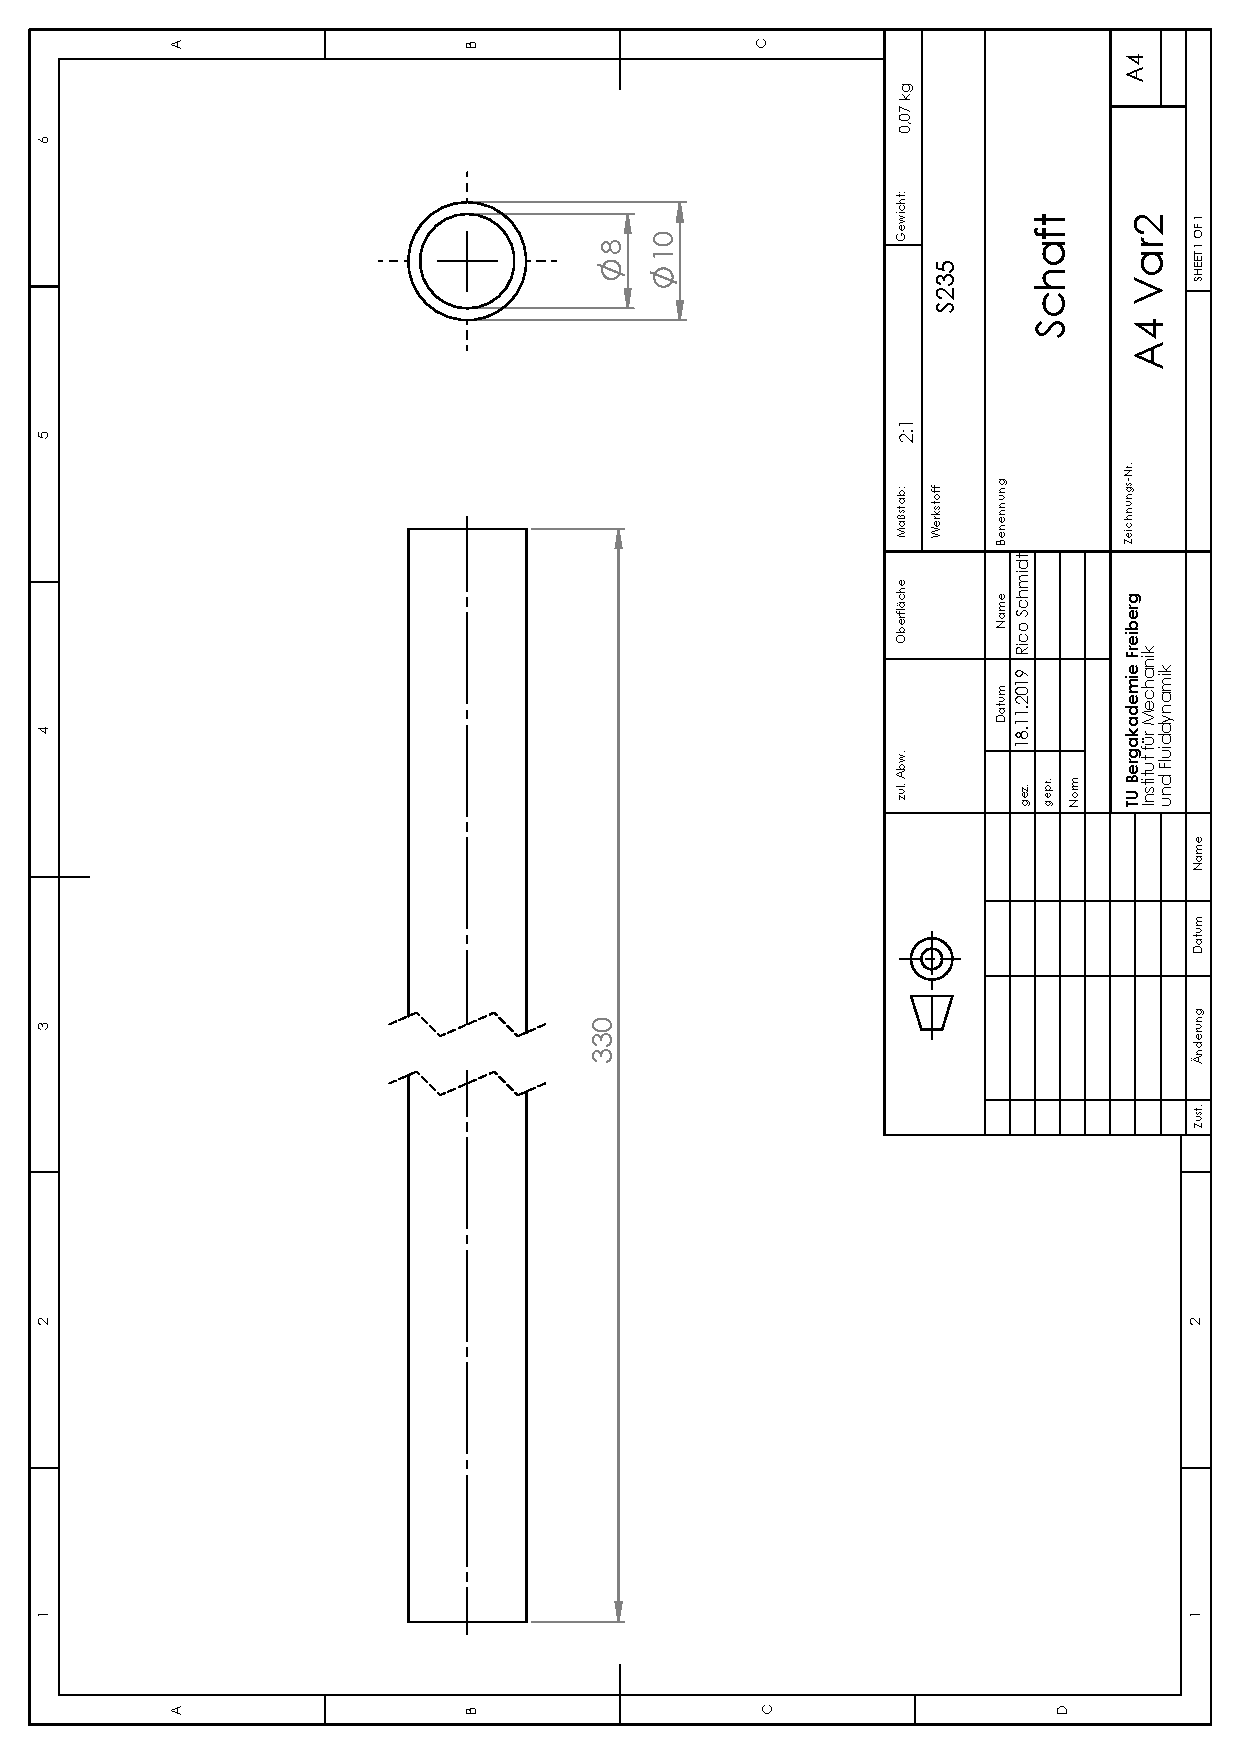
\includegraphics[angle=-90,width=1.0\textwidth]{Anhang/PDFs/Schaft_Ra10mm_Ri8mm}
	
	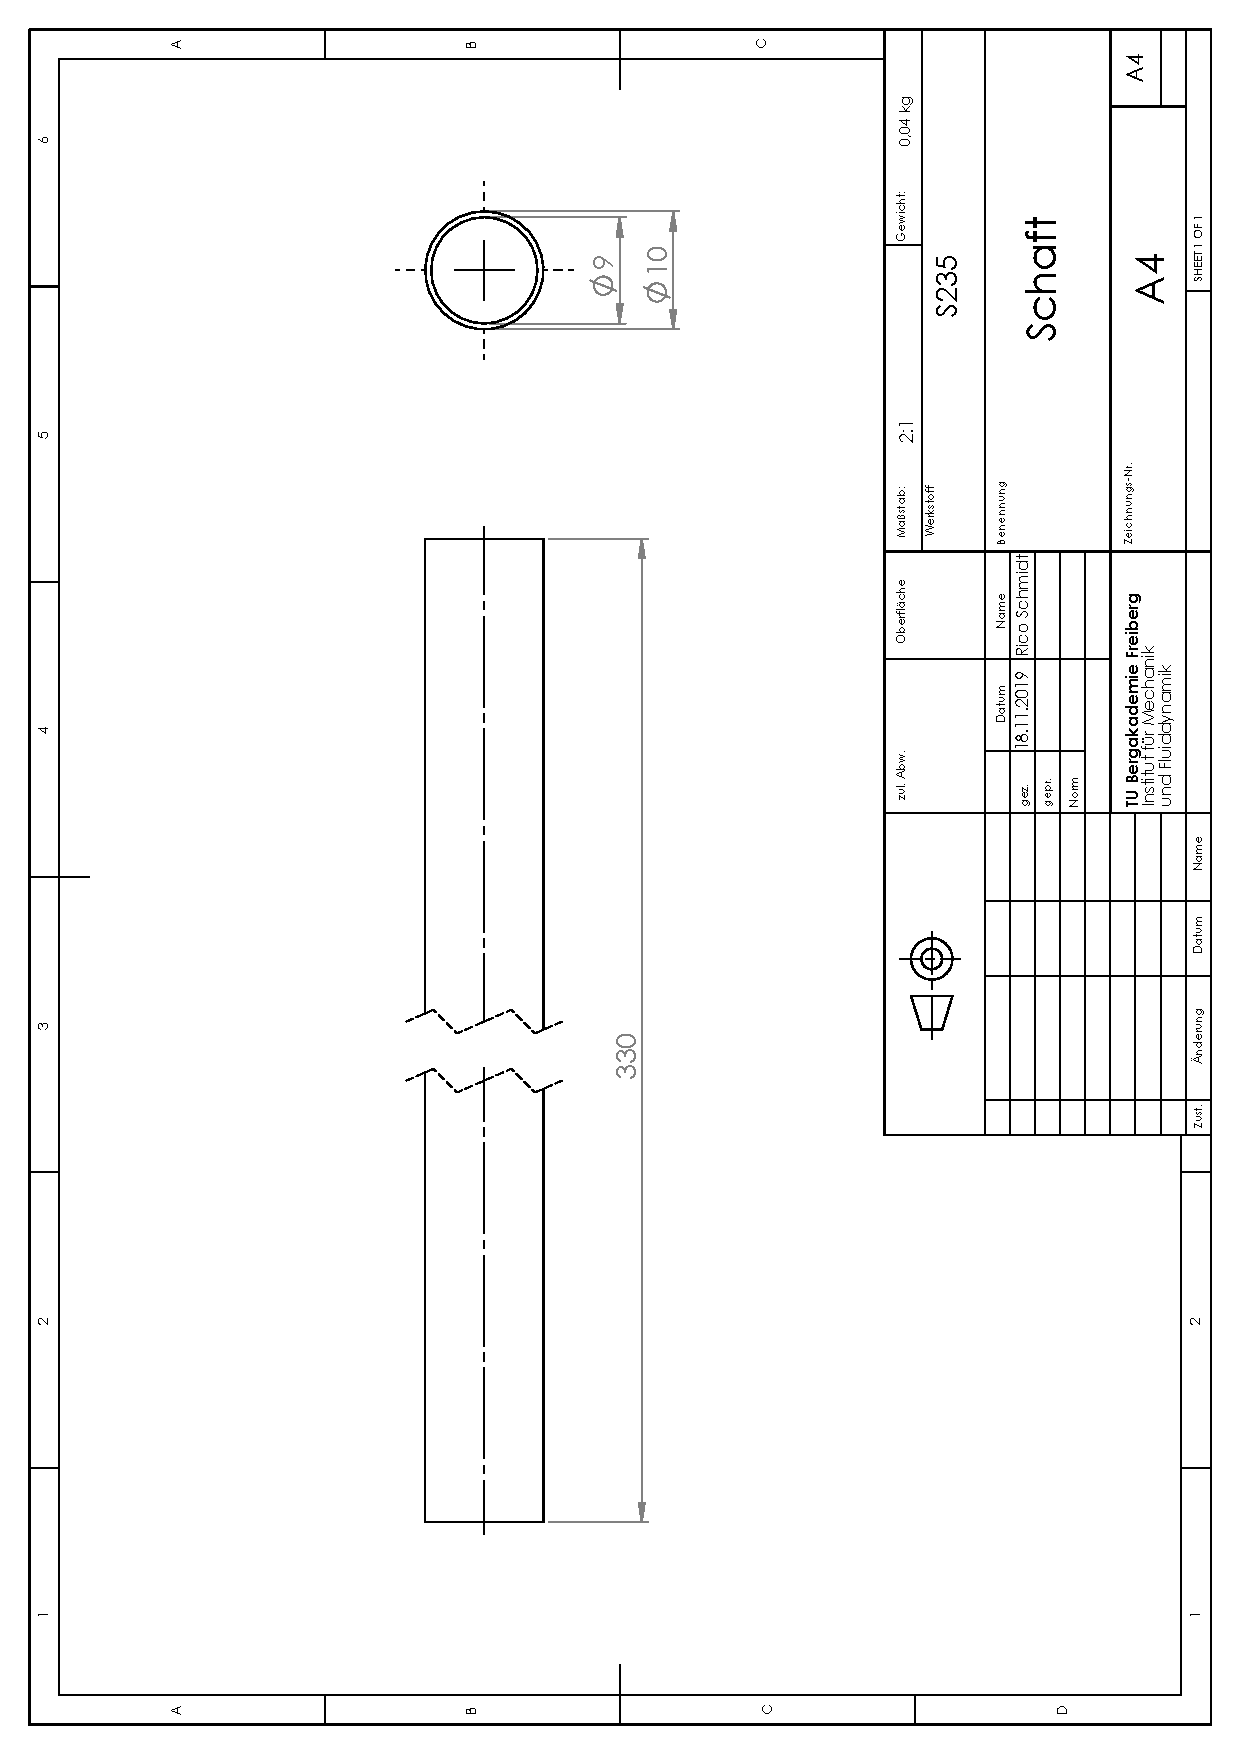
\includegraphics[angle=-90,width=1.0\textwidth]{Anhang/PDFs/Schaft_Ra10mm_Ri9mm}
	
	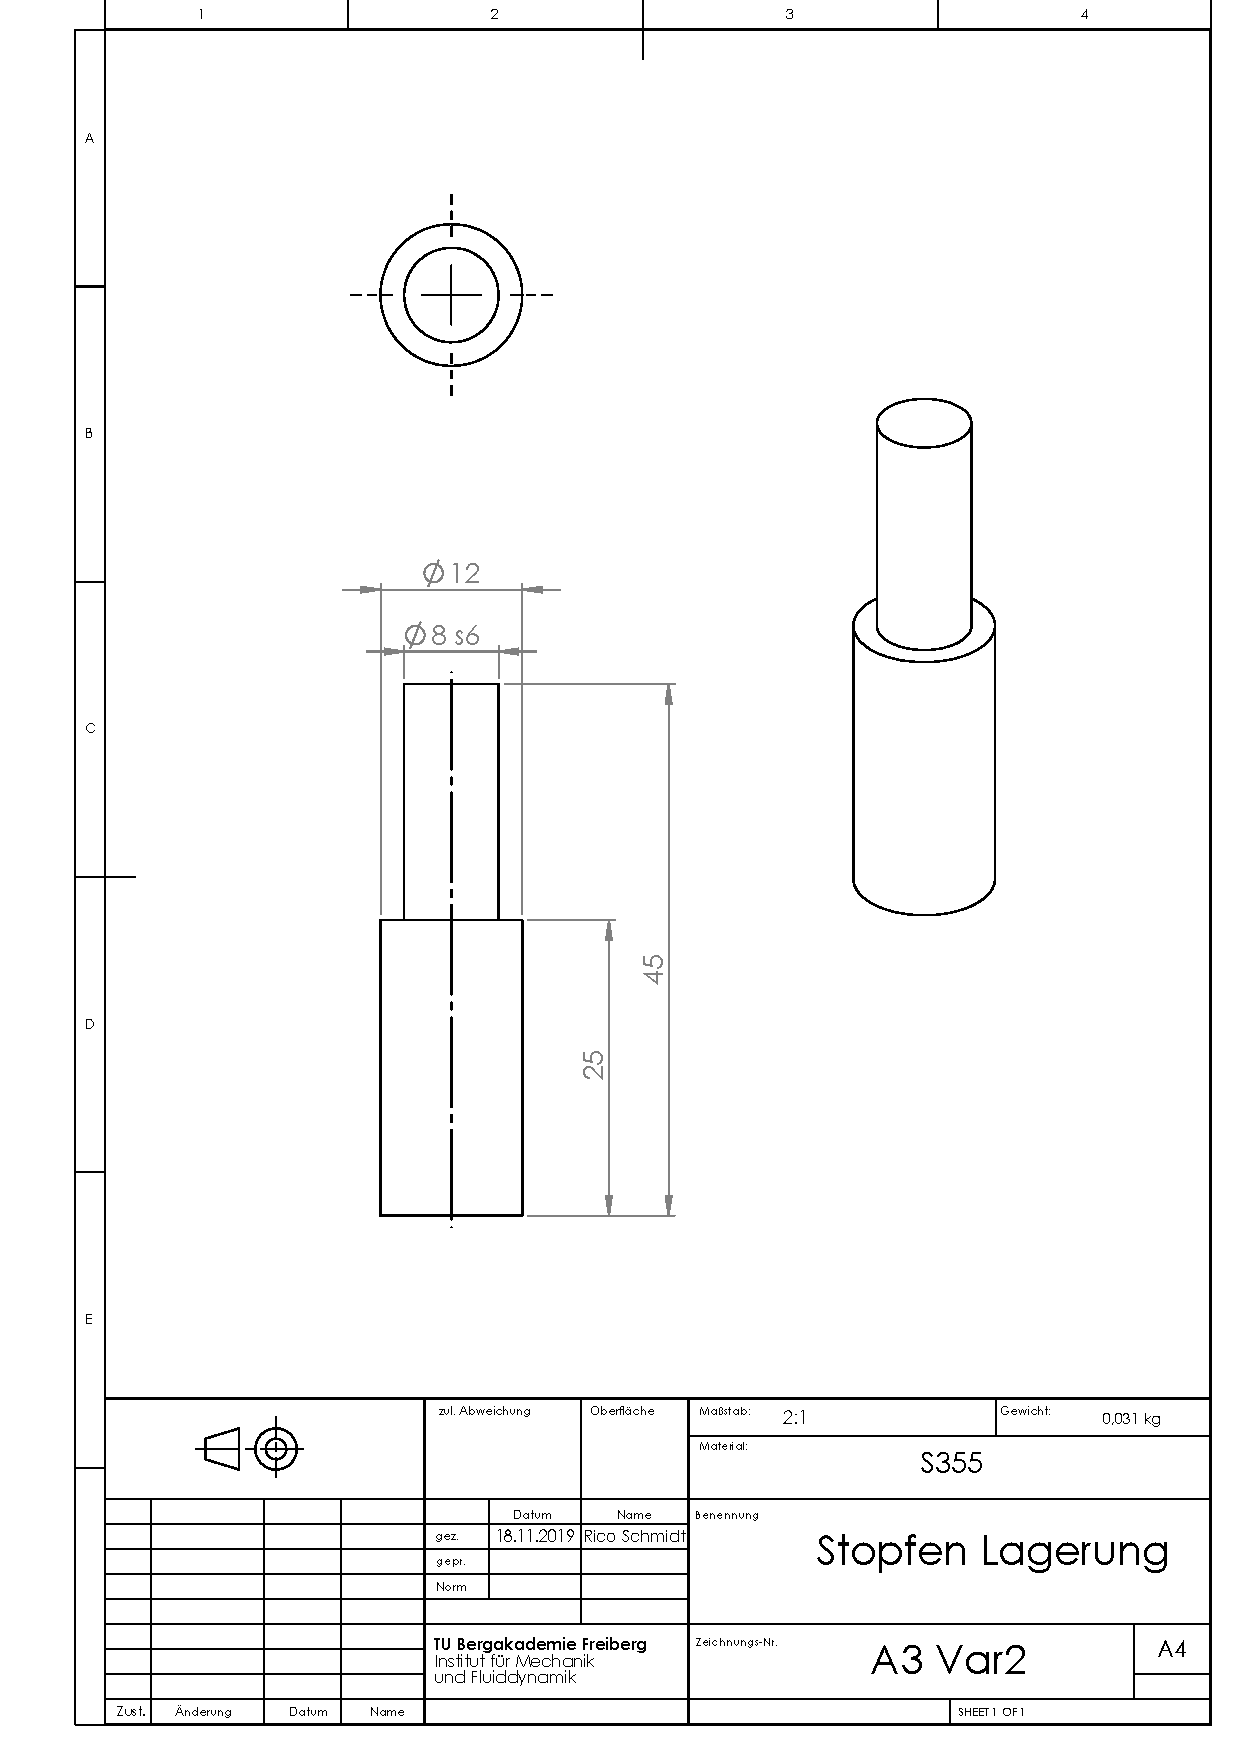
\includegraphics[angle=-90,width=1.0\textwidth]{Anhang/PDFs/Stopfen_Schaft_Lagerung_Var2}
	
	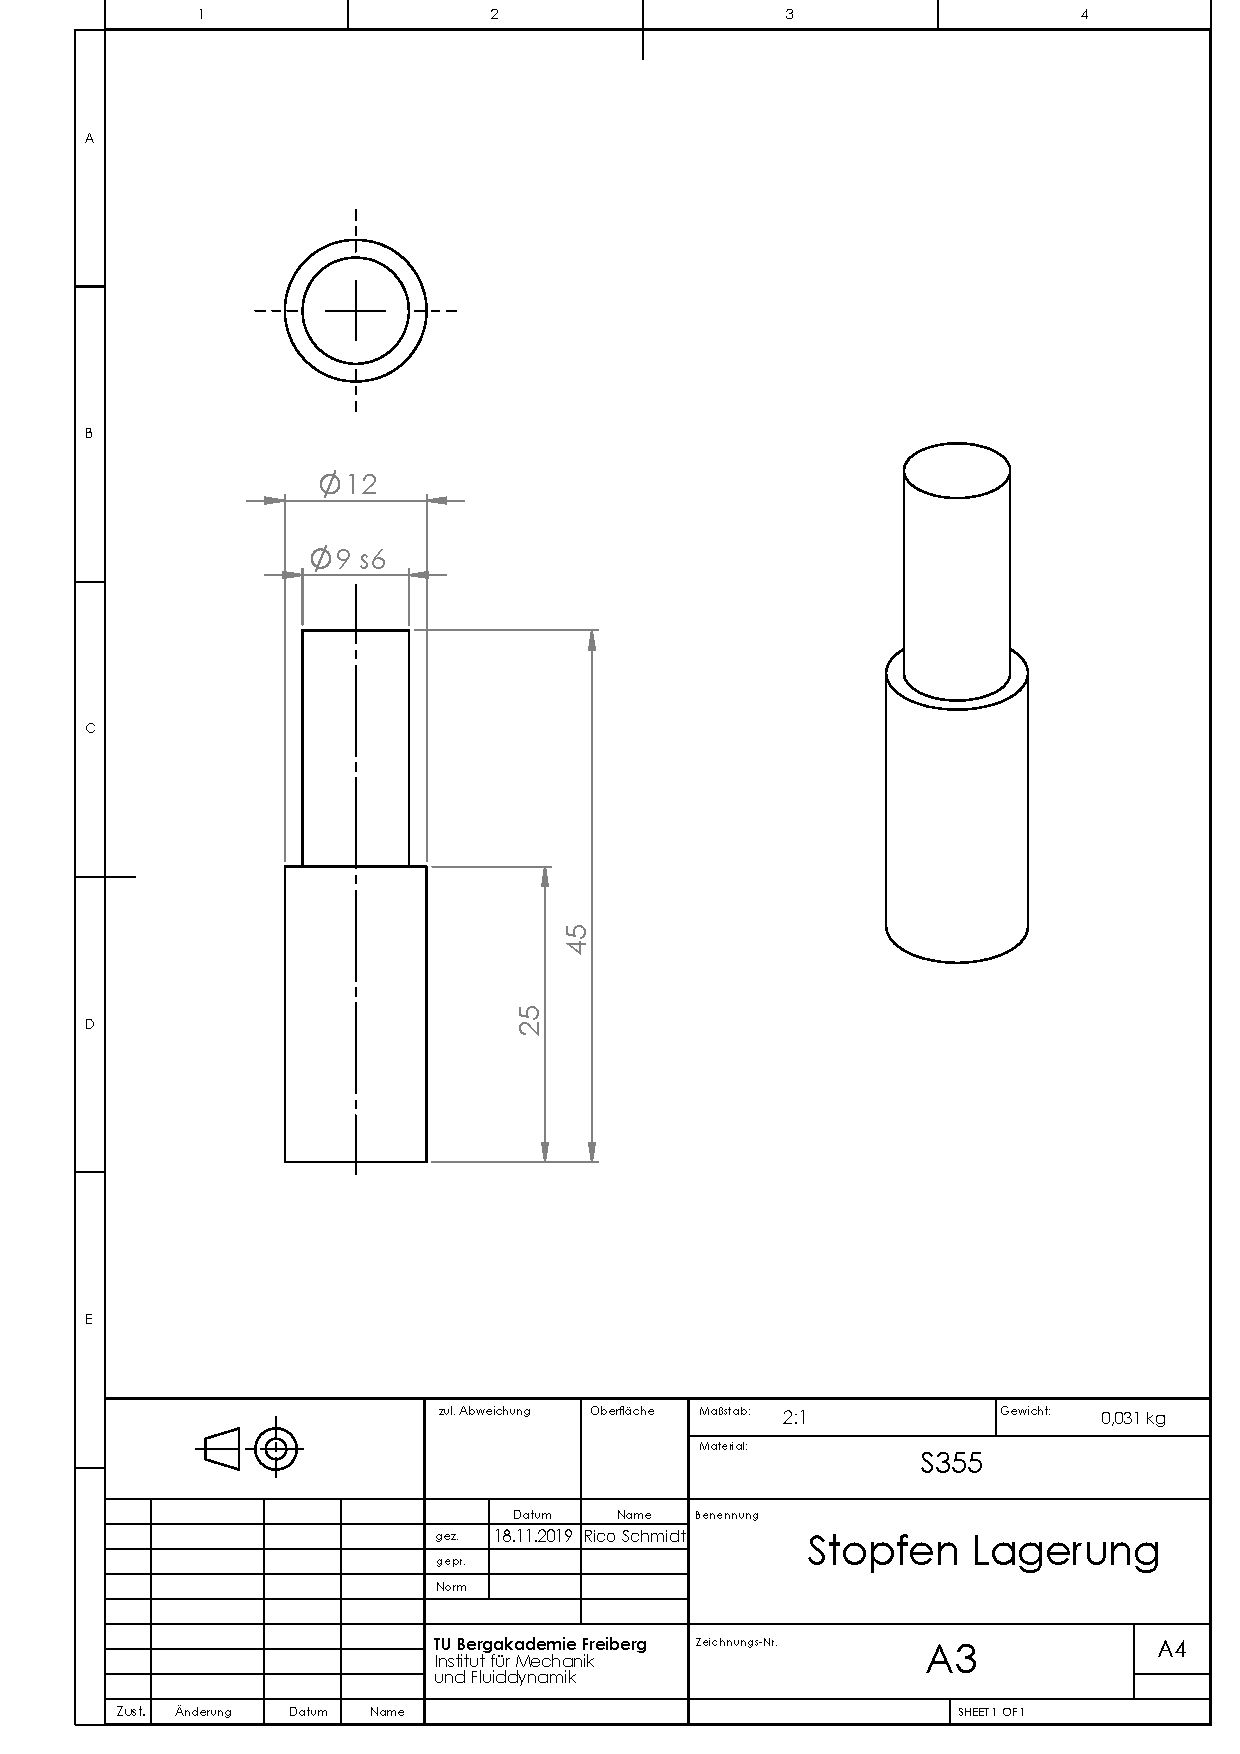
\includegraphics[angle=90,width=1.0\textwidth]{Anhang/PDFs/Stopfen_Schaft_Lagerung}
	
	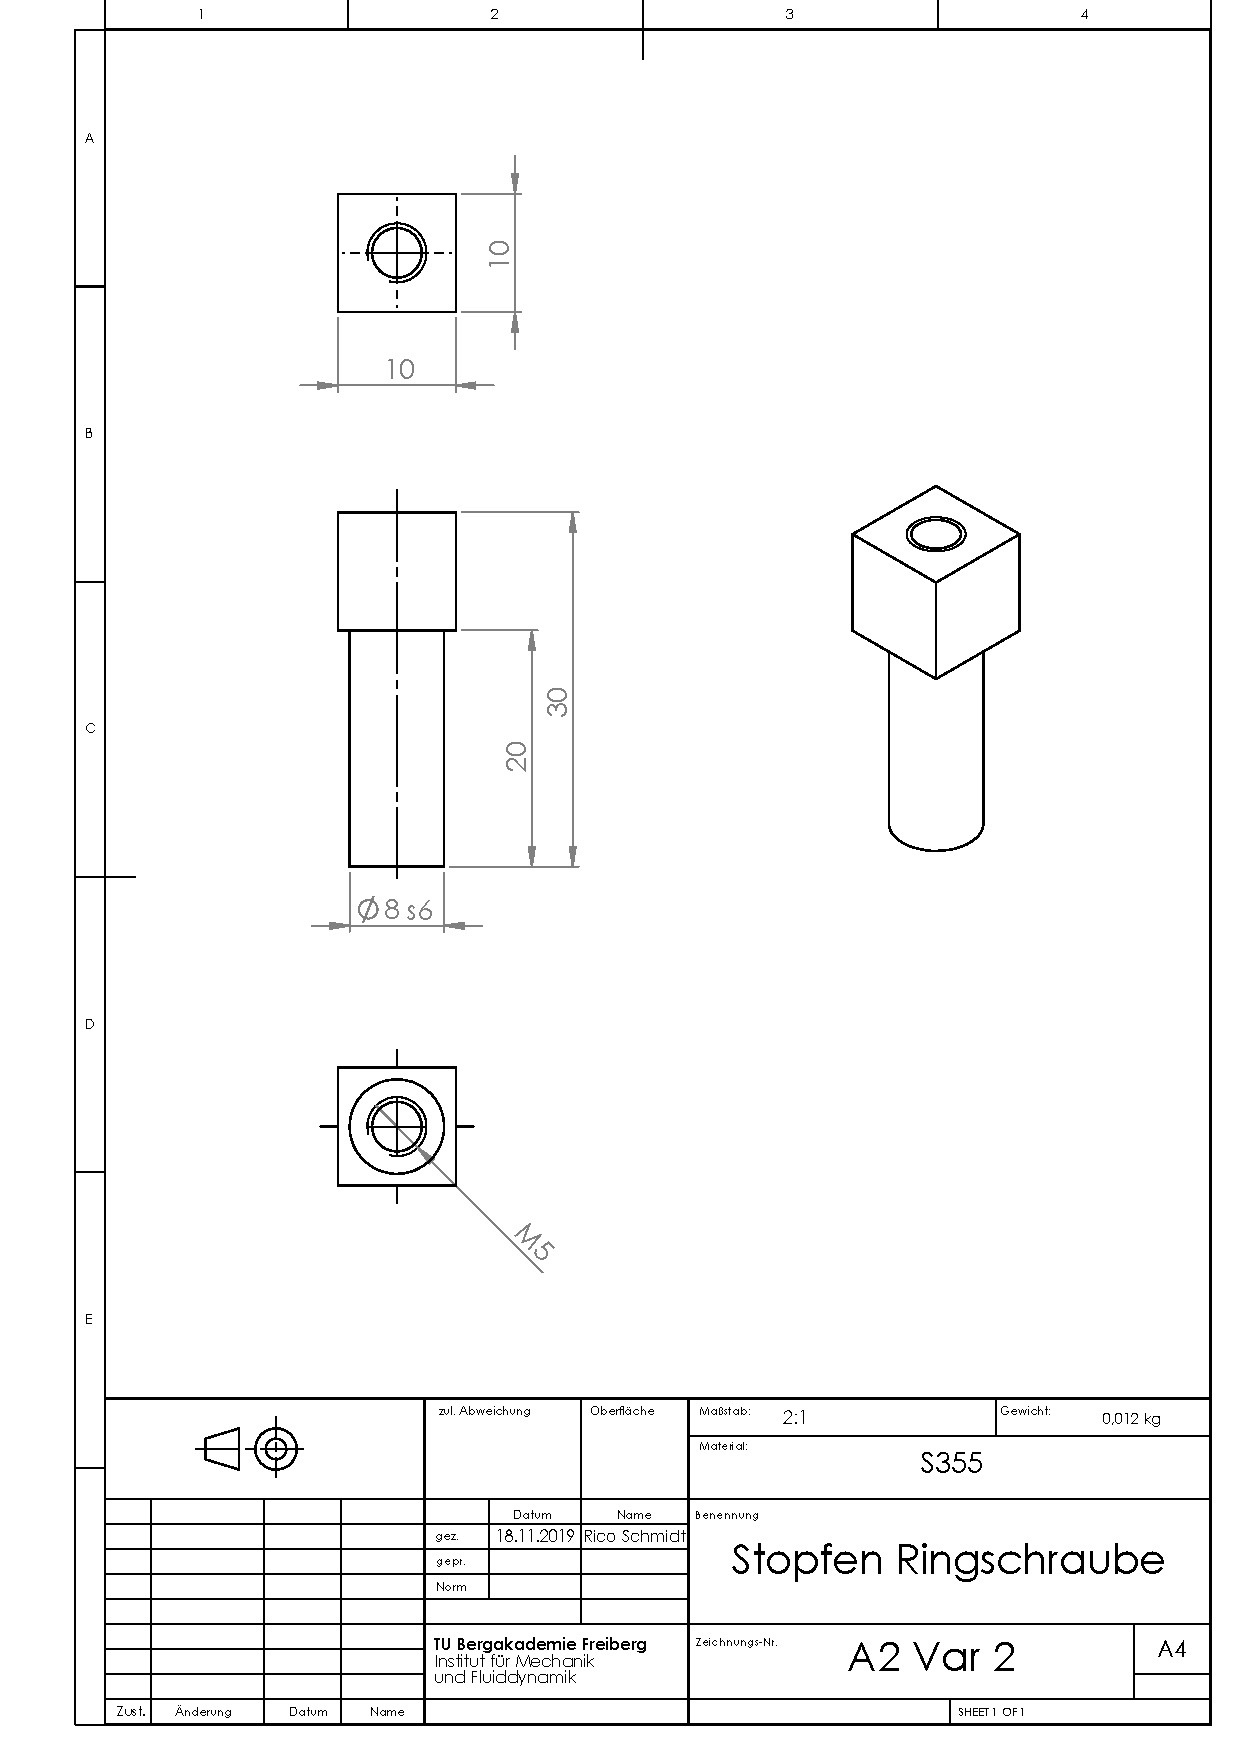
\includegraphics[angle=90,width=1.0\textwidth]{Anhang/PDFs/Stopfen_Schaft_Ringschraube_Var2}
	
	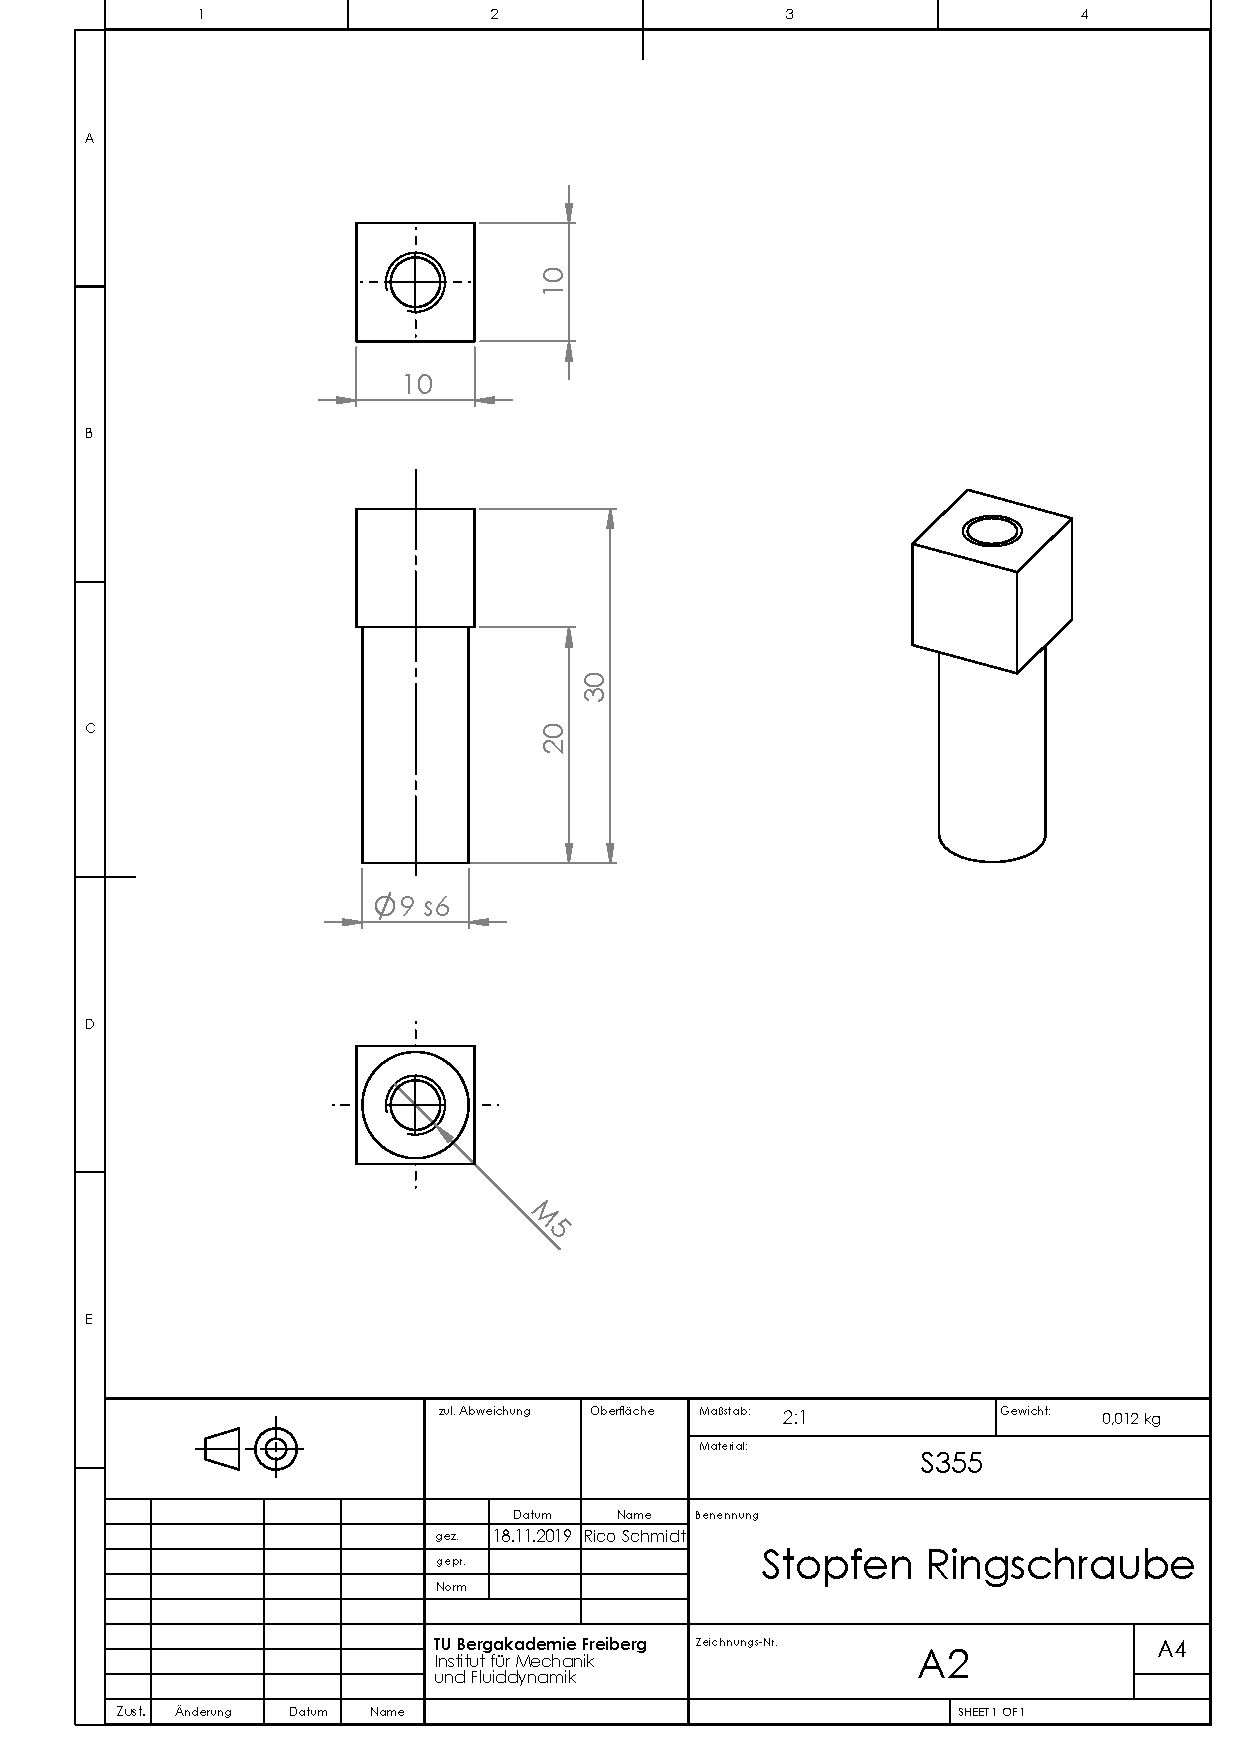
\includegraphics[angle=-90,width=1.0\textwidth]{Anhang/PDFs/Stopfen_Schaft_Ringschraube}
	
	